\documentclass[12pt,a4paper]{article}
\usepackage{times}
\usepackage[utf8]{inputenc}
%\usepackage[english]{babel}
\usepackage[portuguese]{babel}
\usepackage[T1]{fontenc}
\usepackage{cite}
\usepackage{amsmath,amsfonts,amssymb} % pacote matematico
\usepackage{array}
\usepackage{graphicx,wrapfig}
\usepackage{float}
\usepackage{indentfirst}
\usepackage[inline]{enumitem}

\usepackage{psfrag}
\usepackage{pstricks}
\usepackage{epsfig}
\usepackage{url}           % Legenda no texto e na Lista de figuras diferentes. Habilita \cite{} na legenda.

\setlength{\parindent}{1.2cm}
\setlength{\parskip}{.2cm}
\setlength{\oddsidemargin}{0.5cm}    % Há um offset obrigatorio de
\setlength{\evensidemargin}{0.0cm}   % 1 inch do lado esquerdo e no
\setlength{\topmargin}{-1.2cm}       % topo da folha
\setlength{\headsep}{1.0cm}
\setlength{\textwidth}{15.5cm}
\setlength{\textheight}{24.2cm}
\renewcommand{\baselinestretch}{1.2}
\renewcommand{\labelitemi}{\tiny{\textbullet}}  % Define o ícone principal do itemize

%\hyphenation{Trans-ac-tions}


\begin{document}
\pagenumbering{roman}

\begin{titlepage}
\thispagestyle{empty}
\begin{center}
\large{\bf{UFBA - Universidade Federal da Bahia}} \\
\large{\bf{Graduação em Engenharia da Computação}} \\
\end{center}
\vfill

\centering
\textbf{{\LARGE PLANO DE TRABALHO}}  \\ \vspace{0.5cm}
{\LARGE Graduação}
\vfill




\textbf{{\Large Robô de inspeção com visão imersiva}} \\ %\vspace{0.3cm}
%\hrulefill \\
\vfill
\begin{flushleft}
\textbf{Aluno}: Raffaello Salvetti Santos \hfill{}\\
\textbf{Orientador}: --- \hfill{}\\
\textbf{Linha de Pesquisa}: Robótica {\it ou} Sistemas Robóticos \hfill{}\\
\end{flushleft}

\vfill


\vspace{\stretch{1}}
\begin{center}
\large{\bf{\today}}
\end{center}
\end{titlepage}


\pagenumbering{arabic}

\begin{abstract}
	Inspeção de áreas de difícil acesso ou que apresentam perigo, como dutos de ventilação, subestações de energia elétrica e reservatórios de produtos corrosivos, é uma realidade na indústria. O uso de robôs operados remotamente é uma solução que oferece segurança ao operador. O objetivo deste trabalho é desenvolver de um robô remotamente controlado visando eficiência, versatilidade e baixo custo de produção.
\end{abstract}


%---------------------------------------------------------------------------------------------------------
\section{Introdução}
	Dutos de ventilação usado nos sistemas de ar-condicionado estão sujeitos a diversos tipos de danos, dentre os quais pode se listar os entupimentos progressivos devido ao acumulo de poeira e acumulo de pequenos animais mortos. Por normalmente ser um local de pouco acesso, apresentam dificuldades em sua manutenção, favorecendo a proliferação de bactérias e transmissão de vírus.\par
	Sub-estações de energia elétrica oferecem riscos a vida por expor o corpo humano a uma quantidade enorme de energia, apesar de existir norma rigorosa para a realização inspeções preventivas, busca por pontos de oxidação em equipamentos e cabos danificados, acontecem acidentes e algumas vezes com vitimas.\par
	A inspeção de reservatórios de produtos químicos requer uma minuciosa analise estrutural, uma busca por áreas oxidadas e falhas em pontos de solda,  que demanda muito tempo. A exposição a gases e vapores tóxicos, por menor que seja a quantidade, causam riscos a saúde do inspetor.\par
	Os exemplos acima, são apenas algumas das atividades extremamente necessárias no ambiente industrial, que expõem pessoas a riscos de morte e que podem ser evitados através de dispositivos especializados. Os dispositivos usados para esse fim, são robôs equipados com ferramentas adequadas para cada tarefa que podem oferecer um sistema de navegação autônomo ou de controle remoto.

%----------------------------------------------------------------------------------------------------------------------
\section{Objetivo}
	O objetivo deste trabalho é a construção de um robô que pode ser controlado remotamente através de um joystick. O dispositivo oferece uma visão imersiva, através de uma câmera embarcada, que pode funcionar em ambientes iluminados ou com pouca luz e tem eixos livres nas direções horizontal e vertical; possui também uma câmera localizada na parte traseira do robô que permite realizar manobras com mais precisão; É possível coletar informações do ambiente ao redor do robô através de sensores embarcados como: dois sensores de temperatura, um localizado na "cabeça" do robô (sensor laser), que pode ser direcionado, e outro no corpo do dispositivo; sensor de umidade do ar, sensor de partículas em suspensão no ar e etc. As leituras dos sensores são apresentadas na tela de navegação do robô e podem ser enviadas pela rede para um outro operador em tempo de coleta. Através dos dados enviados pela rede, pode ser montado um mapa, com o auxilio de um software especializado, do local onde o robô se encontra.


%---------------------------------------------------------------------------------------------------------
\section{Metodologia}
	Para o desenvolvimento do robô, sera usado uma plataforma feita em alumínio, o chassi, que deverá suportar o peso da bateria, motores, correntes, câmeras e eletrônica necessária para seu funcionamento.\par
	O movimento do robô se dará através de dois motores em conjunto com um par de correntes, acionados por uma placa microcontrolada, especialmente desenhada para esse propósito, que aciona os motores através de PWM\footnote{Modulação por largura de pulso}. A mesma placa que controla os motores de locomoção, controlará os motores que movimentam os motores da câmera frontal. A comunicação entre a placa de controle de motores e o sistema computacional embarcado, um Raspberry PI 1 modelo B, acontecerá através do protocolo $I^2C$. \par
	O software de operação consiste em módulos que serão desenvolvido usando o ROS (Robot Operating System). O desenvolvimento dos módulos ROS será feito de forma independente da parte física do robô pois será usado um simulador de ambiente para esse fim.\par
	Os módulos são: um aplicativo que deverá rodar num celular Android, responsável por mostrar as imagens e sons capturados pelas câmeras embarcadas e fará a ponte de comunicação entre os comandos originados de um joystick bluetooth e a plataforma robótica; um programa que rodará embarcado fará o controle dos motores de locomoção, motores da câmera frontal e a coleta de dados dos sensores; e por fim, um programa que rodará num computador remoto, responsável por armazenar dados, gerenciar a conexão entre os módulos e plotar um mapa virtual do caminho percorrido pelo robô. \par

\subsection{Diagrama de módulos}
\begin{figure}[H]
	\centering
	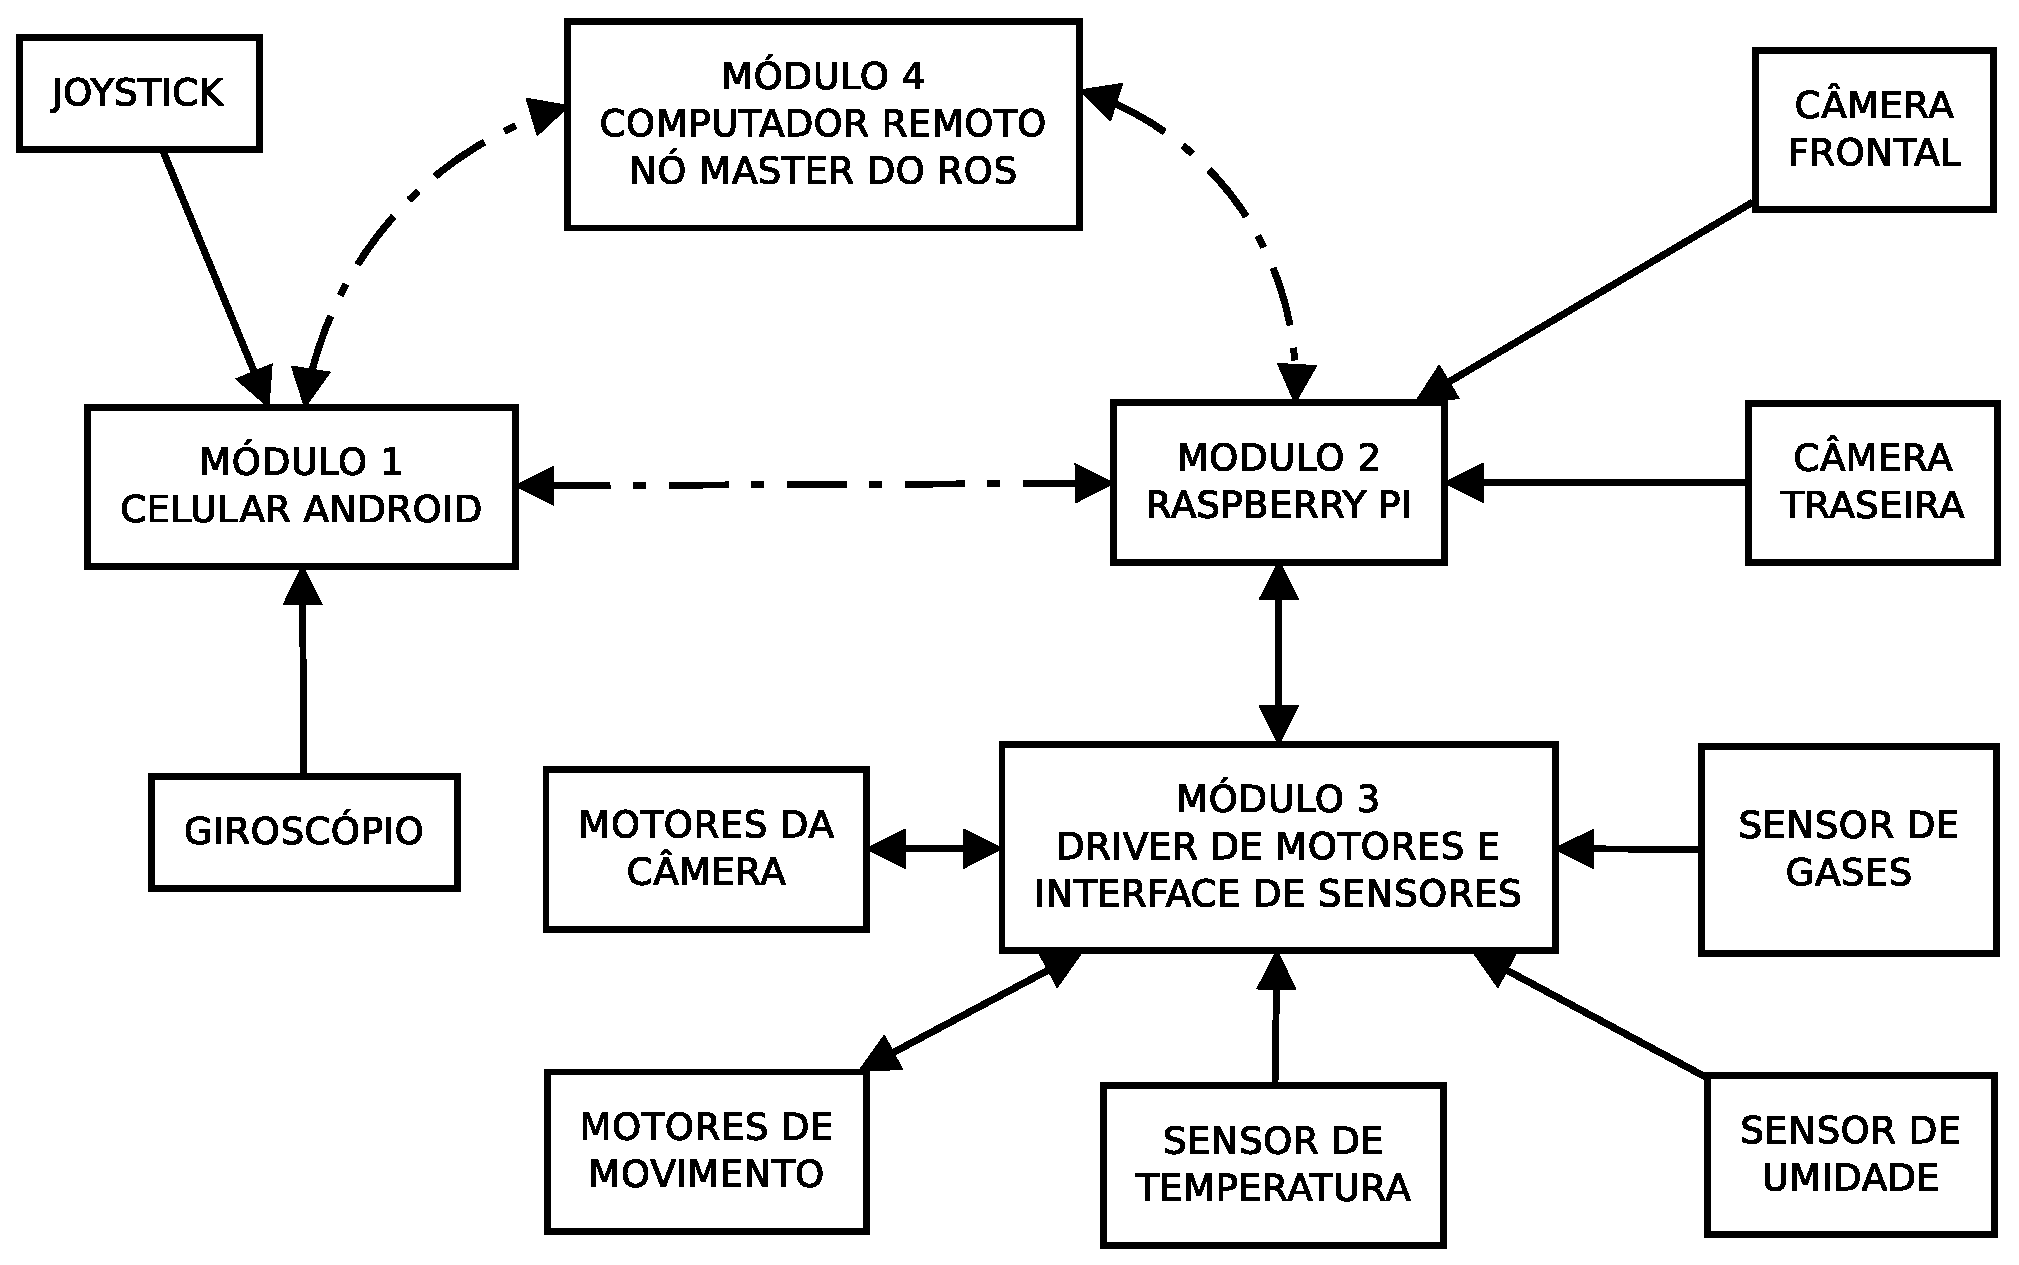
\includegraphics[scale=0.45]{diagrama-modulos} 
	\label{fig:diag-modulos}
	\caption{Diagrama de blocos dos módulos que compõem o robô.}
\end{figure}

\subsection{Descrição dos módulos \label{sec:desc-modulos}}
\begin{enumerate}
\item \textbf{Módulo do Celular Android - Visualização Imersiva\label{mod:celular}}\\
	Esse módulo será um nó do ROS que mostrará as imagens coletadas pelas câmeras embarcadas no robô, módulo \ref{mod:raspi}, e processadas pelo nó master, módulo \ref{mod:ros-master}. Será usado um celular juntamente com um óculos VR como um display para mostrar o vídeo e o som transmitido pelas câmeras, dando a ideia de imersão. O módulo deve enviar os dados do giroscópio do celular afim de movimentar a câmera frontal de acordo com o movimento da cabeça do operador. Um joystick comum, que oferece conectividade bluettoth, será usado para movimentar as esteiras do robô e interagir com as \emph{opções de menu}\footnote{Controle de sensore e luzes.} que aparecem no visor do celular.
\item \textbf{Módulo de Controle Embarcado - Raspberry PI\label{mod:raspi}}\\
	Esse módulo será um nó ROS que rodará num \emph{Raspberry PI 1 modelo B}\footnote{Um micro computador do tipo SOC, do inglês "System on a Chip", ou computador num único chip.}, que possui um processador ARM de 700MHz, 512Mb de memória RAM, 26 GPIO\footnote{Pinos de propósito geral.}, duas portas USB e uma porta Ethernet. Será responsável por enviar os dados de navegação gerados pelo módulo \ref{mod:celular} para uma placa especializada, módulo \ref{mod:motor-driver}. A comunicação entre o módulo \ref{mod:motor-driver} e o Raspberry PI acontecerá pelos pinos GPIO reservados para a comunicação $I^2C$.
\item \textbf{Módulo Driver - Controlador de Motores e Interface de Sensores\label{mod:motor-driver}}\\
	O módulo drive será uma placa de circuito impresso que possui um microcontrolador AVR ou PIC com periféricos, memória e quantidade de pinos suficientes para realizar suas tarefas. A placa driver terá as seguintes funções: \begin{enumerate*} \item monitorar a tensão da bateria; \item fazer a regulação da tensão de 12V para 5V, tensão que alimenta o Raspberry PI; \item acionar os dois motores das esteiras e os dois  motores da câmera frontal; \item coletar dados dos diversos sensores embarcados; \item controlar as luzes usadas na iluminação do ambiente\end{enumerate*}. A placa possuirá um display indicativo para depuração e status do robô, e um conector do tipo header de duas linhas com 26 pinos, usado para a conexão com os GPIOs do Raspberry PI.
\item \textbf{Módulo Principal - ROS Master\label{mod:ros-master}}\\
	O módulo \ref{mod:ros-master} deverá rodar em um computador com um certo poder de processamento. Para o caso em questão, será um notebook com requisitos de hardware suficientes para rodar o ROS e ser o nó master, rodar processamentos do Open CV para o reconhecimento de imagens e recurso suficiente para plotar um mapa virtual do trajeto executado pelo robô. 
\end{enumerate}

\subsection{Conhecimento Necessário}
	Para contruir os módulos listados na seção \ref{sec:desc-modulos}, se faz necessário os seguintes conhecimentos:
\begin{enumerate}[noitemsep]
	\item Eletrônica Geral
	\item Microcontroladores
	\item Protocolos de Comunicação (SPI e I2C)
	\item Fontes de Alimentação
	\item Supressão de Ruido (Interferência Eletromagnética)
	\item Acionamento de Motores
	\item Sistemas de Transmissão Mecânica (Corrente de Transmissão)
	\item Sistema Operacional Linux
	\item Sistema Operacional de Robôs - ROS
	\item Sistema Operacional Android
	\item Linguagens de Programação (C e Java)
	\item Android SDK (Cardboard SDK)
	\item Redes de Computadores (Ethernet e Bluetooth)
	\item Visão Computacional (Open CV)
\end{enumerate}

\subsection{Modelo 3D}
\begin{figure}[H]
	\centering
	\includegraphics[scale=0.45]{modelo} 
	\label{fig:diag-modulos}
	\caption{Modelo 3D do robô.}
\end{figure}

%---------------------------------------------------------------------------------------------------------
\section{Resultados Esperados}
Explicite qual será a utilidade da pesquisa, a quem deverá importar os resultados, o que será produzido e o que se espera, enfim, com a elaboração do seu trabalho. 


%---------------------------------------------------------------------------------------------------------
\section*{Referências Bibliográficas}
% OBSERVAÇÃO: A seção de referências deve ser gerada automaticamente usando os comandos \cite{} do LaTex. Recomenda-se o uso do padrão IEEE para citações, conforme abaixo.

\bibliographystyle{IEEEtran}
\bibliography{bibliografia}

\end{document}
